\section*{Ziel}
Im folgenden Versuch soll die Eigenschaften eines Lasers untersucht werden. 
Dazu wird unteranderem die Wellenlänge, die Polarisation, das Modenspektrum und die Intensitätsverteilung in der Ebene senkrecht zur Ausbreitungsrichtung betrachtet.
Geprüft wird Stabilitätsbedingung des Resonators, 2 TEM-Moden des Lasers, sowie die Beugung an einem Strichgitter.
\section{Theorie}
\subsection{Funktionsweise eines Lasers}
Ein Laser (Light Amplification by Stimulated Emission of Radiation) besteht grundsätzlich aus drei verschiedenen
Komponenten. Diese befassen das Lasermedium, ein Resonator und eine Pumpquelle. Das Lasermedium bestimmt dabei durch optische Übergänge
das Strahlenspektrum des Lasers, sodass dieser monochromatisches Licht hoher Intensität und Kohärenz erreicht.
Der Resonator bildet die Grundlage für eine selbstanregende Oszillation, sodass eine optische Rückkopplung des ausgestrahlten Laser entsteht und somit wiederholt
durch das Lasermedium geleitet wird. Energie wird dem System über die Pumpquelle hinzugefügt, sodass es zur einer Inversion kommt.
Umfassend lässt sich sagen, dass das Strahlungsfeld in jener Art und Wiese mit dem Lasermedium wechselwirkt, sodass das einfallende Licht verstärkt wird.
\subsection{Zwei-Niveau-System}
Zunächst wird das Zwei-Niveau-System betrachtet. Auch wenn sich dieses für den Laser nicht nutzen lässt, soll zunächst zum
Verständnis der Zustandssysteme beitragen.\\
Bei dem Helium-Neon-Laser handelt es sich um enen Gasentaldungslaser. Das enthaltende Medium hat dabei
zwei mögliche Energiezustände $E_1$ und $E_2$ in denen sich jeweils $N_1$ und $N_2$ Teilchen befinden (Besetzungszahl).
Durch die Pumpquelle können die Teilchen nun auf das höhere Energieniveau $E_2$ angeregt werden.
Folgende drei Prozesse, dargestellt in Abbildung \ref{fig:3wege} können dabei auftreten.
\subsubsection*{Anregung durch Absorbtion}
Dabei bringt ein Photon, welches mindestend die Energie $\Delta E=E_2-E_1$ besitzt, das Teilchen vom Grundzustand in den angeregten Zustand.
\subsubsection*{Spontane Emission}
Das angeregte Atom emittiert spontan ein Photon in beliebige Richtung und kehr somit in den Grundzustand zurück.
\subsubsection*{Induzierte Emission}
Ein Photon mit der Energie zwischen angeregtem Zustand und Grundzustand löst einen Übergang im Medium aus. Das entstehende stimulierte Photon
bewegt sich in die selbe Richtung, bei gleicher Energie, Phasenlage und P0larisation.

\begin{figure}
    \center
    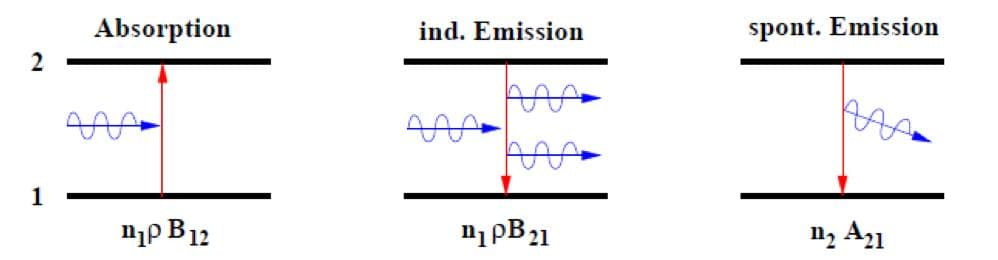
\includegraphics[width=0.8\textwidth]{bilder/3wege.jpg}
    \caption{Absorbtion und Emission schematisch Dargestellt für ein Strahlungsfeld $\rho(\nu)$ in einem Zweizustandssystem \cite{anleitung}}
    \label{fig:3wege}
\end{figure}
\label{sec:theorie}

Für die absorbierten und emittierten Photonen gilt $\omega=\frac{\Delta E}{\hbar}$ und die Different $\Delta N$ bezeichnet man als Inversion.
Durch die Anregung folgt eine zeitliche Änderung der Besetzungszahlen $N_1$ und $N_2$, die sich schreibt lassen als
\begin{align}
    \frac{dN_1}{dt}&=-N_1\rho B_{12}+N_2\rho B_{21} + N_2 A_{21}\\
    \frac{dn_2}{dt}&=+N_1\rho B_{12}-N_2\rho B_{21} - N_2 A_{21}= -\frac{dN_1}{dt}.
\end{align}
Dabei spiegelt $A_{21}$ den Einsteinkoeffizienten für spontane Emission, $B_{12}$ für Absorbtion und $\rho$ die spektrale Strahldickte im Resonator wieder.
Da gilt
\begin{align}
    N&=N_1+N_2{,}\\
    \Delta N &= N_2-N_1{,}\\
    B_{12}&=B_{21}:=B{,}\\
    A_{21}&:=A{,}   
\end{align}
folgt somit
\begin{equation}
    \frac{d\Delta N}{dt}=-2B\rho\Delta N + AN-A\Delta N.
\end{equation}
Da aufgrund des thermischen Gleichgewichtes (Maxwell-Boltzmann-Verteilung) mehr Teilchen den Grundzustand besetzten und somit maximal eine 
Gleichbesetztung der beiden Energiezustände erreicht werden kann, lässt sich ein Laser durch ein Zweizustandssystem nicht realisieren. Kurz gesagt,
es lässt sich keine Inversion (angeregter Zustand iegt öfter vor als Grundzustand) erreichen.
Dies ist allerdings notwendig, damit die stimulierte Emission häufiger als die induzierte Emission auftritt und somit die gewünschte Verstärkung des Strahlungsfeldes auftritt.

\subsection{Höhere Niveau-Systeme}
Das dargelegt Problem des Zwei-Niveau-Systems kann durch das Einführen weiterer Niveaus gelöst werden ($E_3$ bei einem Drei-Niveau-System und $E_0$ bei Vier-Niveau-System).
Dabei gilt $E_0\leq E_1 \leq E_2 \leq E_3$. Gepumpt wird dabei weiterhn vom tiefsten zum höchsten Niveau, wobei die Übergänge von $E_3$ nach $E_2$ und $E_1$ nach $E_0$ schneller ablaufen als von $E_2$ nach $E_1$.
Dies liefert $N\approx N_0+N_2$ und $\Delta N \approx -N_2$.
Für die zuvor angegebenen Raten folgt daher,
\begin{align}
    \frac{dN_1}{dt}&\approx 0\\
    \frac{dN_2}{dt}&=+N_0\rho B_{12}-N_2A_{12}
\end{align}

\subsection{Der Resonator}
Da die gewünschte Verstärkung exponentziell von der Länge des Laufweges im ativen Lasermedium abhängt, ist die Nutzung eines optischen Resonators sinnvoll.
Realsisert wird dieser durch zwei sich gegenüberliegenden totalreflektierenden (geringe Transmission) Spiegeln (dargestellt in Abbildung \ref{fig:resonator}).
Dadurch wird eine Verstärkung durch stimulierte Emission erzeugt, welche größer als die Abschwächung der Absorbtionsverluste oder Auskopplung sind.

\begin{figure}
    \center
    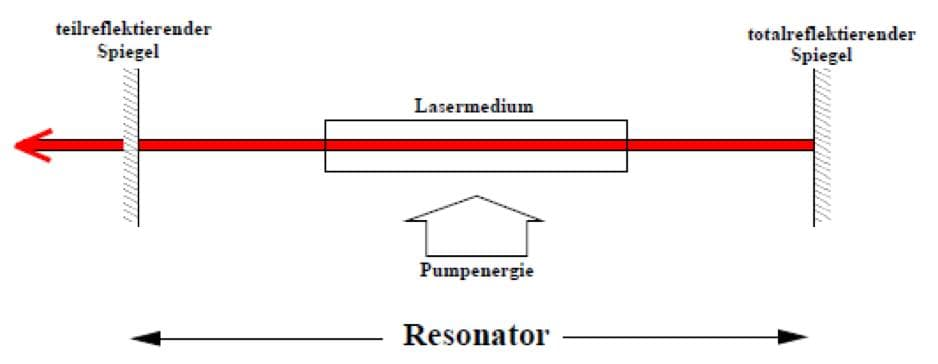
\includegraphics[width=0.8\textwidth]{bilder/resonator.jpg}
    \caption{Schematische Darstellung des Resonators mit zwei totalreflektierenden Speigeln \cite{anleitung}.}
    \label{fig:resonator}
\end{figure}

Unterschieden werden die Resonatoren durch die eingesetzten Spiegel. So besteht ein planparalleler Resonator aus zwei planparallelen Spiegeln und ein sphärischer Resonator aus zwei sphärischen Spiegel.
Fallen die Spiegelbrennpunkte zusammen, so werden besonders geringe Verluste erreicht, man spricht von einem konfokalen Resonator.\\
Für die notwendige Verstärkung durch induzierte Emission ist eine selsterregende Oszillation nötig, welche an die Stabilitätsbedingung
\begin{equation}
    0 \leq g_1 g_2\leq 1
    \label{eq:stabil}
\end{equation}
geknüpft ist. Dabei beschreibt $g_i$ den Resonatorparameter durch
\begin{equation}
    g_i=1-\frac{L}{r_i}
\end{equation}
mit der Resonatorlänge $L$ und den Krümmungsradien der Spiegel $r_i$.\\
\subsection{Polarisation}
Ein linearer Polarisator kann genutzt werden, um die polarisation eines Lasers zu bestimmen. Dabei wird lediglich das Licht der entsprechend eingestellten Polarisation transmittiert.
Über die Veränderung der Intensität kann somit auf die Polrisation geschlossen werden, sie verhält sich gemäß des Gesetz von Malus
\begin{equation}
    I=I_0\cos^2(\theta)
\end{equation}
wobei $\theta$ den Winkel zwischen der optischen Achse des Polarisators und der Polarisationsrichtung und $I_0$ die Anfangsintensität der Welle beschreibt

\subsection{TEM-Moden}
Da für die Wellenlänge $\lambda<<L$ gilt, folgen daher mehrere Resonanzbedingungen für eine stehende Welle im Resonator.
Sodass die Moden des Resonators mit TEM$_{\text{lpq}}$ bezeichnet werden. Wobei $q$ die longitudinale Mode und $l$ und $p$
die transversalen Knotenpunkte in x- und y-Richtung angeben, welche durch Unebenheiten in den Spiegeln auftreten.\\
Höhere Moden haben dabei größere Verluste zu verzeichnen als niedriege Moden. Für die Verlustfreiste Mode TEM$_{00}$ folgt die  gaußverteilte
Intensität mit
\begin{equation}
    I(r)=I_0\exp(\frac{2r^2}{w^2})
\end{equation}
wobei $r$ der Abstand zur optischen Achse, $I_0$ das Intensitätsmaximum und $w$ die Strahl divergenz nach $w=\lambda w_0/\pi$ ist.
\subsubsection{Longitudinale Moden}
Eine stehende Welle bildet sich demnach für
\begin{equation}
    n\frac{\lambda}{2}=L
\end{equation}
aus, wobei $n$ eine ganzzahlige Zahl mit $n>0$ ist. Die Anzahl der Wellenberge im Resonator sind demnach $q=n/2$.
Mit der Grundfrequenz $w_0$, der Teilchenmasse $m$, der Temperatur $T$ und der Boltzmannkonstante $k_B$ lässt sich das Geschwindigkeitsprofil $\sigma_w$
und der Abstand der Resonanzfrequenzen $\Delta w$ bestimmen.
\begin{align}
    \sigma_w&=\frac{w_0}{c}\sqrt{\frac{k_B T}{m}}\\
    \Delta w &=\frac{c}{2L}
\end{align}
Die statisch verteilte Raumbewegung der Gasmoleküle bildet dabei die Verstärkungskurve aus, die einer Einhüllender in Form einer Gaußverteilung gleicht.
\subsubsection{Transversale Moden}
Bei Störung der Resonatorsymmetrie treten transversale elektromagnetische Moden auf. Diese kann aufgrund von Verunreinigungen auf
der Spiegeloberfläche ausgelost werden. Die auftretenden Interferenzen leifern zweidimensionale Amplitudenverteilungen.
Wie bereits erwähnt spiegelt der Index TEM$_{\text{lp}}$ (bzw. TEM$_{\text{xy}}$) die inder x- und y-Richtung befindlichen Knotenpunkte wieder.
Für das Auslösen bzw. Verstärken einer gewissen Mode kann z.B. eine Blende (für TEM$_{00}$) oder ein dünner Draht (für TEM$_{10}$) verwendet werden.
\begin{figure}
    \center
    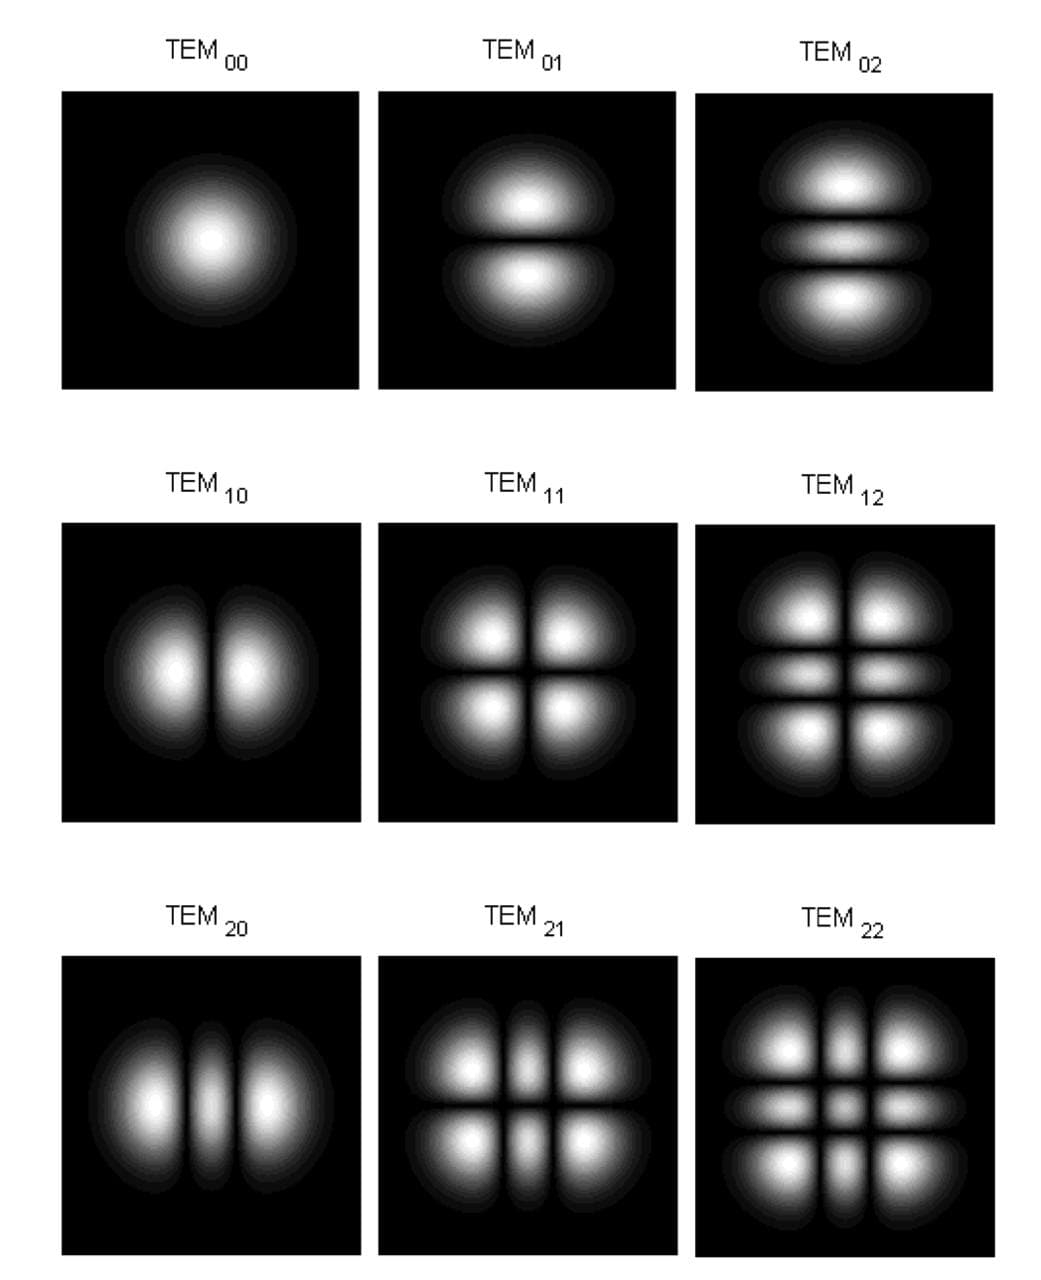
\includegraphics[width=0.7\textwidth]{bilder/moden.jpg}
    \caption{TEM$_{\text{lp}}$-Moden mit entsprechendem Intensitätsprofil.}
\end{figure}